\documentclass[border=10pt]{standalone}

\usepackage{tikz}
\usepackage{tikzsymbols}
\usetikzlibrary{calc,patterns,shapes.geometric}

\def\centerarc[#1](#2)(#3:#4:#5){\draw[#1] ($(#2)+({#5*cos(#3)},{#5*sin(#3)})$) arc (#3:#4:#5);}

\begin{document}
	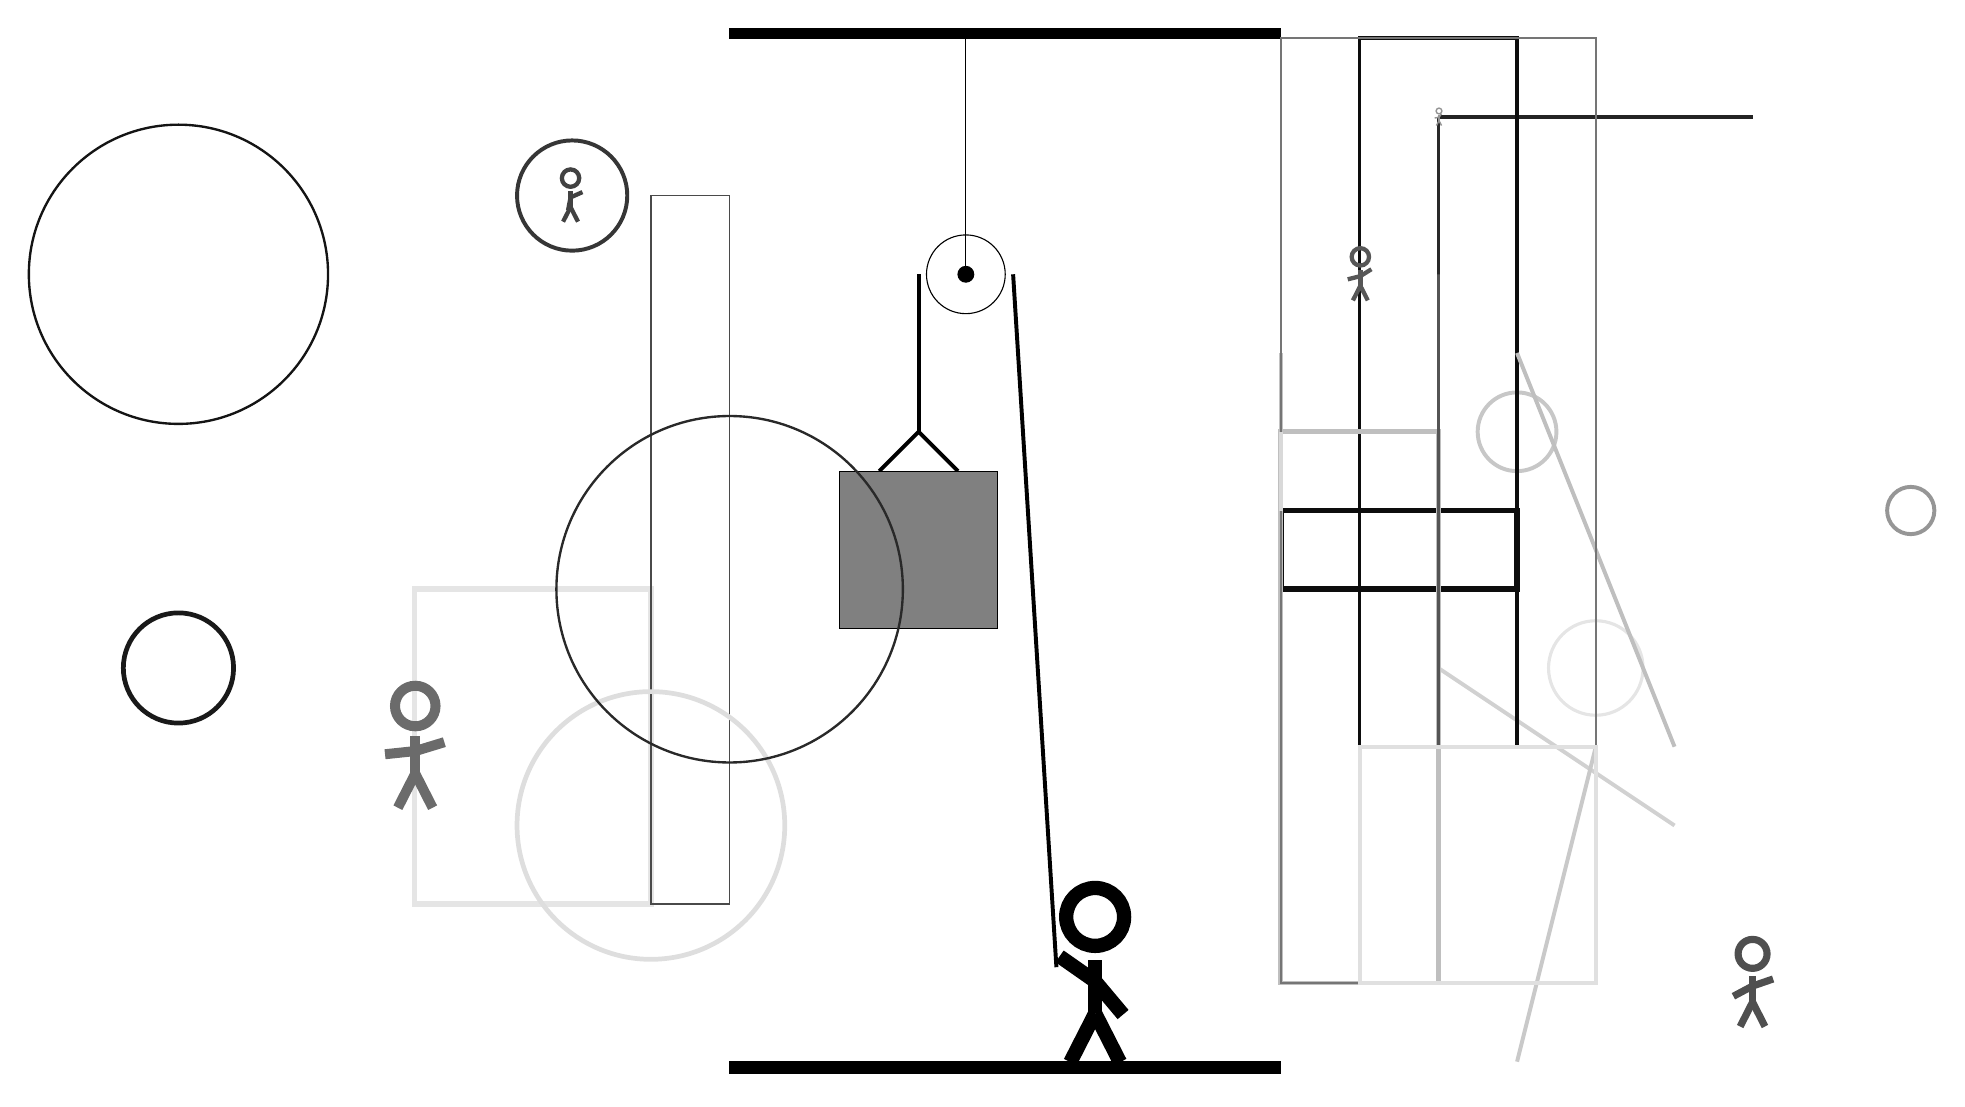
\begin{tikzpicture}
		%%%%% START %%%%%
		
		\draw[fill=black] (-2, 10) rectangle (5, 10.125);
		
		\draw (1, 7) circle (0.5);
		\draw[fill=black] (1, 7) circle (0.1);
		\draw (1, 10) -- (1, 7);
		
		\draw[line width=0.5mm] (-0.1, 4.5) -- (0.4, 5.0) -- (0.9, 4.5);
		\draw[fill=black!50] (-0.6, 4.5) rectangle (1.4, 2.5);
		
		\draw[line width=0.5mm] (0.4, 7) -- (0.4, 5.0);
		\centerarc[line width=0.5mm](1, 7)(0:180:0.6);
		\draw[line width=0.5mm](1.6, 7) -- (2.15, -1.8);
		
		\draw[line width=0.4mm, color=black!84] (7, 4) rectangle (7, 9);
		
		\draw[line width=0.7mm, color=black!10] (-3, 3) rectangle (-6, -1);
		\node[line width=0.3mm, color=black!74] at (-4, 8) {\Strichmaxerl[3][79][24]};
		\draw [line width=0.5mm, color=black!22](8, 5) circle (0.5);
		\draw[line width=0.5mm, color=black!18](7, 2) -- (10, 0);
		\draw[line width=0.5mm, color=black!24](5, 2) -- (5, 6);
		
		\draw[line width=0.5mm, color=black!21](8, -3) -- (9, 1);
		\draw[line width=0.2mm, color=black!71] (-2, 8) rectangle (-3, -1);
		\draw [line width=0.4mm, color=black!10](9, 2) circle (0.6);
		
		\draw[line width=0.5mm, color=black!86](7, 9) -- (11, 9);
		
		\node[line width=0.5mm, color=black!42] at (7, 9) {\Strichmaxerl[1][7][57]};
		\draw[line width=0.4mm, color=black!95] (6, 1) rectangle (8, 10);
		\draw[line width=0.5mm, color=black!25](8, 6) -- (10, 1);
		\draw[line width=0.7mm, color=black!95] (5, 3) rectangle (8, 4);
		\draw [line width=0.3mm, color=black!92](-9, 7) circle (1.9);
		\draw[line width=0.6mm, color=black!25] (5, 5) rectangle (7, -2);
		
		\draw [line width=0.6mm, color=black!13](-3, 0) circle (1.7);
		\draw[line width=0.3mm, color=black!54] (5, -2) rectangle (9, 10);
		\draw[line width=0.4mm, color=black!67] (7, 1) rectangle (7, 7);
		\draw [line width=0.6mm, color=black!90](-9, 2) circle (0.7);
		\draw [line width=0.5mm, color=black!79](-4, 8) circle (0.7);
		\draw [line width=0.3mm, color=black!84](-2, 3) circle (2.2);
		\node[line width=0.3mm, color=black!66] at (6, 7) {\Strichmaxerl[3][14][32]};
		\draw[line width=0.5mm, color=black!12] (6, 1) rectangle (9, -2);
		\draw[line width=0.5mm, color=black!15](5, 5) -- (5, 4);
		
		\node[line width=0.4mm, color=black!58] at (-6, 1) {\Strichmaxerl[7][6][17]};
		
		\draw [line width=0.5mm, color=black!41](13, 4) circle (0.3);
		\node[line width=0.3mm, color=black!69] at (11, -2) {\Strichmaxerl[5][28][19]};
		
		\node at (2.6, -1.9) {\Strichmaxerl[10][-35][-50]};
		
		\draw[fill=black] (-2, -3) rectangle (5, -3.15);
		
		%%%%% END %%%%%
	\end{tikzpicture}
\end{document}